\documentclass[a4paper,11pt]{article}

%% Language and font encodings
\usepackage[spanish,english]{babel}
\usepackage[utf8]{inputenc}
\usepackage[T1]{fontenc}
%% Sets page size and margins
\usepackage[a4paper,top=2cm,bottom=2cm,left=2cm,right=2cm,marginparwidth=2cm]{geometry}
%% Useful packages
\usepackage{amsmath}
\usepackage{graphicx}
\usepackage[colorinlistoftodos]{todonotes}
\usepackage[colorlinks=true, allcolors=blue]{hyperref}
\setlength{\marginparwidth}{2cm}
\usepackage{authblk}
\usepackage[none]{hyphenat}

\setlength{\parindent}{1em}
\usepackage{indentfirst}
\setlength{\parskip}{3pt}

\usepackage[T1]{fontenc}
\usepackage[utf8]{inputenc}
\usepackage{graphicx}
\usepackage{xcolor}

\renewcommand\familydefault{\sfdefault}
\usepackage{tgheros}

\usepackage{amsmath,amssymb,amsthm,textcomp}
\usepackage{enumerate}
\usepackage{multicol}
\usepackage{tikz}

\usepackage{geometry}
\geometry{left=25mm,right=25mm,%
bindingoffset=0mm, top=20mm,bottom=20mm}


\linespread{1.3}

\newcommand{\linia}{\rule{\linewidth}{0.5pt}}

% code listing settings
\usepackage{multicol}
\usepackage{listings}
\lstset{
    language=Python,
    basicstyle=\fontsize{7pt}{7pt}\ttfamily,
    aboveskip={0.5\baselineskip},
    belowskip={0.5\baselineskip},
    extendedchars=true,
    breaklines=true,
    tabsize=2,
    prebreak=\raisebox{0ex}[0ex][0ex]{\ensuremath{\hookleftarrow}},
    frame=lines,
    showtabs=false,
    showspaces=false,
    showstringspaces=false,
    keywordstyle=\color[rgb]{0.627,0.126,0.941},
    commentstyle=\color[rgb]{0.133,0.545,0.133},
    stringstyle=\color[rgb]{01,0,0},
    numbers=left,
    numberstyle=\tiny,
    stepnumber=1,
    numbersep=10pt,
    escapeinside={\%*}{*)},
    frameround=ftff,
    frame=single,
}

%%%----------%%%----------%%%----------%%%----------%%%

\title{INFORME PROYECTO ALM}
\author{}

\begin{document}
\graphicspath{./images/} 

\vfill
{
    \maketitle
    \vspace{1cm}
    \begin{center}
    \begin{tabular}{c c c}
        Victor Callejas Fuentes &  David Alarcón & Jose Mira\\
        \small 4CO11 & 4CO11 & 4CO11 \\
        \small viccalfu@inf.upv.es & viccalfu@inf.upv.es & jomigar4@inf.upv.es \\
    \end{tabular}
    \end{center}
    \vspace{1cm}
    \begin{abstract}
        \center En este documento se recoge el código desarrollado así como los resultados obtenidos y decisiones tomadas durante la realización de las práctias de laboratorio.
    \end{abstract}

    \newpage
}

{
\hypersetup{linkcolor=black}
\tableofcontents
\newpage
}

\section{Tarea 1 - Distancias de edición}
Implementaión de distancias de edición entre cadenas de forma iterativa y mediante programación dinámica

\subsection{Distancia de Levensthtein}
Considerando las operaciones de inserción, borrado y sustitución con coste = 1.

\begin{lstlisting}[caption=Algoritmo distancia de levenshtein]
    mat = matriz(x, y)
    res = np.zeros(shape=(len(x)+1,len(y)+1))
    for i in range(0,len(x)+1):
        for j in range(0,len(y)+1):
                if i==0 or j==0:
                    res[i,j] = res[i,j] + i + j
                else:
                    res[i,j] = min(
                        mat[i-1,j-1] + res[i-1,j-1],
                        1 + res[i-1,j],
                        1 + res[i,j-1]
                    )

    return res[len(x),len(y)]
\end{lstlisting}


\subsection{Distancia de Damerau-Levensthtein restringida}
Se añade la operación de trasposición. En esta versión una vez intercambiados dos
símbolos, éstos no se pueden utilizar en otras operaciones de edición.

\begin{lstlisting}[label={list:first},caption=Sample Python code -- Damerau-Levensthtein restringido]
    INF = len(x) + len(y)

    mat = matriz(x, y)
    res = np.zeros(shape=(len(x)+1,len(y)+1))

    for i in range(0,len(x)+1):
        for j in range(0,len(y)+1):
                if i==0 or j==0:
                    res[i,j] = res[i,j] + i + j
                elif i == 1 or j == 1:
                    res[i,j] = min(
                        mat[i-1,j-1] + res[i-1,j-1],
                        1 + res[i-1,j],
                        1 + res[i,j-1],
                    )
                else:
                    res[i,j] = min(
                        mat[i-1,j-1] + res[i-1,j-1],
                        1 + res[i-1,j],
                        1 + res[i,j-1],
                        1 + res[i-2,j-2] + (mat[i-2,j-1] + mat[i-1,j-2]) * INF
                    )
    return res[len(x),len(y)]
\end{lstlisting}

\vfill
\subsection{Distancia de Damerau-Levensthtein intermedia}
Considerando las operaciones de trasposición cuando:
\begin{equation}
    |u| + |v| 	\leqslant cte \Leftarrow cte = 1
\end{equation}
\begin{lstlisting}[label={list:first},caption=Damerau-Levensthtein intermedio]
    M = init_matriz(x, y)

    for i in range(1, len(x) + 1):
        for j in range(1, len(y) + 1):

            if x[i - 1] == y[j - 1]:
                initActual = min(M[i-1, j] + 1, M[i, j-1] + 1, M[i-1][j-1])
            else:
                initActual = min(M[i-1, j] + 1, M[i, j-1] + 1, M[i-1][j-1] + 1)

            if j > 1 and i > 1 and x[i - 2] == y[j - 1] and x[i - 1] == y[j - 2]:
                M[i,j] = min(initActual, M[i-2][j-2] + 1)
            elif j > 2 and i > 1 and x[i-2] == y[j-1] and x[i-1] == y[j-3]:
                M[i,j] = min(initActual, M[i-2][j-3] + 2)
            elif i > 2 and j > 1 and x[i - 3] == y[j-1] and x[i-1] == y[j-2]:
                M[i,j] = min(initActual, M[i-3][j-2] + 2)
            else:
                M[i,j] = initActual

    return M[len(x), len(y)]
\end{lstlisting}

\subsection{Testing}
En el código se encuentra una test flag, por defecto activada, para que a la hora de importar este módulo se compruebe que el comportamiento de los algortimos es el adecuado.

\newpage
\section{Distancias de edición con thresholds}

\begin{lstlisting}[label={list:second},caption=Sample Bash code.]
#! /bin/bash
python stage1.py
echo "Stage I done!"
python stage2.py
echo "Stage II done!"
python stage3.py
echo "Stage III done!"
\end{lstlisting}

Lorem ipsum dolor sit amet, consectetur adipiscing elit, sed do eiusmod tempor incididunt ut labore et dolore magna aliqua. Ut enim ad minim veniam, quis nostrud exercitation ullamco laboris nisi ut aliquip ex ea commodo consequat. Duis aute irure dolor in reprehenderit in voluptate velit esse cillum dolore eu fugiat nulla pariatur. Excepteur sint occaecat cupidatat non proident, sunt in culpa qui officia deserunt mollit anim id est laborum.

\newpage
\section{Tarea 3 - Metodo Suggest}

\subsection{TO BE CONTINUED}
wertewrt

\newpage 
\section{Tarea 4 - Implementación mediante Tries}

\subsection{TO BE CONTINUED}
erwter

\newpage 
\section{Tarea 5 - Estudio experimental}

{\color{red}Realizado por Víctor Callejas} 

En esta parte se pide realizar un estudio experimental de medidas de tiempo para determinar qué
versiones de las anteriores son las más eficientes para unos datos concretos
\subsection{Condideraciones}
Utilizamos dos diccionarios (castellano e inglés) ambos contruidos mediante el texto de la declaración de derechos humanos.

Sobre estos creamos múltiples diccionarios con las N([20,100,500,2500]) palabras más frecuentes. Para ello sobrecargamos el constructor de la clase Suggest de maneara que acepte un path al corpus y un set de palabras ya creado.

Sobre cada uno de estos se crean N consultas([10,50,250,500,2500]). Estas son palabras pertenecientes al diccionario sobre las que se realizan unas perturbaciones aleatorias.

\begin{lstlisting}[caption=Función para crear perturbaciones aleatorias]
def perturbar(word):

    word = list(word)

    n_ops = random.randint(0, min(len(word)-1,MAX_PERTURBACIONES))

    for _ in range(0,n_ops):

        op = random.randint(0, 3)

        if op == 0: # borrar
            idx = random.randint(0,len(word)-1)
            word = word[:idx] + word[(idx+1):]
        elif op == 1: # cambiar
            idx = random.randint(0,len(word)-1)
            char = chr(random.randint(ord('a'),ord('z')+1))
            word[idx] = char
        elif op == 2: # trasposicion
            idx = random.randint(0,len(word)-2)
            tmp = word[idx]
            word[idx] = word[idx+1]
            word[idx+1] = tmp

    return "".join(word)
\end{lstlisting}

Estas consultas se realizan con todos los algoritmos desarrollados en las tareas previas.

Utilizamos el mismo diccionario y consultas con todos los algoritmos (datos apareados).

Repetimos 3 veces la medición de tiempo de cada algoritmo para cada talla de diccionario y consultas para luego poder explorar los resultados y ver que son consistentes y válidos.
\begin{lstlisting}[caption=medición de tiempos]
    start = time.time()
                        
    for consulta in tqdm(consultas,total=len(consultas),leave=False,desc='Consultas: ',position=4):
        _ = iss.suggest(consulta,distance=alg,threshold=STATIC_THRESHOLD)

    end = time.time()
    elapsed = end - start
\end{lstlisting}

\subsection{Resultados}

Una vez ejecutado el programa y realizado la medición de tiempos observamos que los tiempos medidos en las diferentes repeticiones con los mismos datos son parecidos, para ello obtenemos la media y desviaciones estándar.

Por ejemplo: para inglés, con talla de diccionario 20, talla de consultas 10 y el algoritmo Iterative intermediate obtenemos una media de 0.028734 y desviación estándard de 0.000572. Por lo que concluimos que los datos son válidos y procedemos a realizar la media de las diferentes repeticiones.

Realizamos el mismo procedimiento para los dos idiomas, inglés y castellano, observamos que el tiempo medidio con los mismos parametros son parecidos. Por lo tanto concluimos que los diferentes algoritmos se comportan igual en ambos idiomas y procedemos a realizar la media de ambas mediciones.

Finalmente, obtenemos para cada algoritmo una medición para cada talla de diccionario y talla de consulta.

Los resultados obtenidos muestran que los algoritmos más rápidos son Trie Levenhtein, seguido de Trie restricted.

\begin{figure}[h]
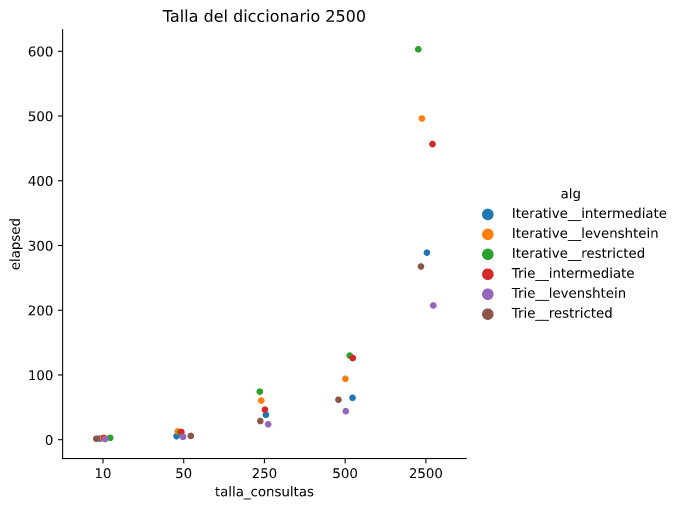
\includegraphics[width=15cm, height=10cm]{images/grafico.png}
\centering
\end{figure}

\newpage 
\section{Tarea 6 - Integración proyecto SAR}
{\color{red}Realizado por David Alarcón, Víctor Callejas y José Mira}

\subsection{Implementación}
Hemos creado un método al cual se le pasa el índice de noticias, un término, una distancia y un threshold. Este método devuelve la lista de indices de noticias en el que aparecen los términos que cumplen las condiciones de distancia especificadas, en base al termindo de búsqueda.

\begin{lstlisting}[caption=Método buscar índices de noticias con palabras aproximadas]
def buscar_aproximados(index, term, distancia, threshold):
    suggesterObject = suggester(list(index.keys()))
    return list(dict.fromkeys(
        itertools.chain.from_iterable(
        [index[word] for word, _ in suggesterObject.suggest(term, distancia, threshold).items() ]
            )
        ))
\end{lstlisting}

Para que esto funcione con nuestro searcher hemos añadido un try catch a la hora de acceder al índice de una palabra si se produce un KeyError esto significa que el término no está en el índice por lo que hemos de recurrir a sus terminos sugeridos en base a la distancia especificada.

\begin{lstlisting}[caption=Método buscar índices de noticias con palabras aproximadas]
try:
    l1 = index[term]
except KeyError:
    l1 = buscar_aproximados(index, term, distancia, threshold) if aproximada else  []
\end{lstlisting}

El funcionamiento de nuestro suggester puede variar dependiendo de los parámetros que se le pasen a este.
\begin{itemize}
    \item \emph{--index{\_}file} El index file a usar.
    \item \emph{--ql{\_}file} El nombre del arcivo que contiene la lista de queries que queremos ejecutar.
    \item \emph{--distancia} La distancia que se quiere usar por defecto se usa levenshtein ya que es con la que mejor resultados hemos obtenido en la tarea 5.
    \item \emph{--threshold} El threhold que se desea usar.
    \item \emph{--query} La query que se le desea pasar al buscador en caso de que se prediera pasar una query en vez de un archivo de queries.
\end{itemize}

Todas las distancias de nuestro buscador se ejecutan con la configuración de tipo Trie ya que han sido las que mejor resultados nos han dado en la tarea5.

\newpage

\subsection{Testing}
{\color{red}Realizado por David Alarcón}

Se incluye un archivo tester.py el cual contrasta los resultados obtenidos por nuestro searcher con los resultados referncia de poliformat.

Para ejecutar los test desde el directorio tarea 6 ejecutamos:

\begin{lstlisting}[language=bash]
    $ python tester.py
\end{lstlisting}

Si este no printea nada por consola indica que ha ejecutado todos los tests de forma correcta.

\newpage

\end{document}